\section{Times have changed}

\begin{frame}[t]{First microprocessor}
\begin{columns}[T]
  \begin{column}{.7\textwidth}
    \begin{itemize}
      \item Intel 4004 (1971).
        \begin{itemize}
          \item \textmark{Application domain}: Calculators.
          \item \textmark{Technology}: 10,000 nm.
          \vfill
          \item \textenum{Data}:
            \begin{itemize}
              \item 2300 transistors.
              \item 13 mm2
              \item 108 KHz
              \item 12 Volts
            \end{itemize}
          \vfill
          \item \textenum{Features}:
            \begin{itemize}
              \item 4-bits data.
              \item Data-path in one cycle.
            \end{itemize}
      \end{itemize}
    \end{itemize}
  \end{column}
  \begin{column}{.3\textwidth}
    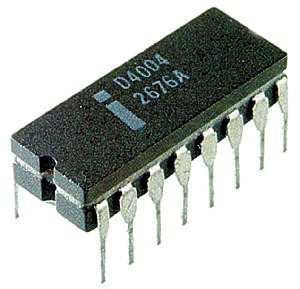
\includegraphics[width=.8\textwidth]{images/intel-4004.jpg}\\
    \begin{tiny}
      \emph{Intel 4004} photo by Rostislav Lisovy\\
    \end{tiny}
    \vspace{1em}
    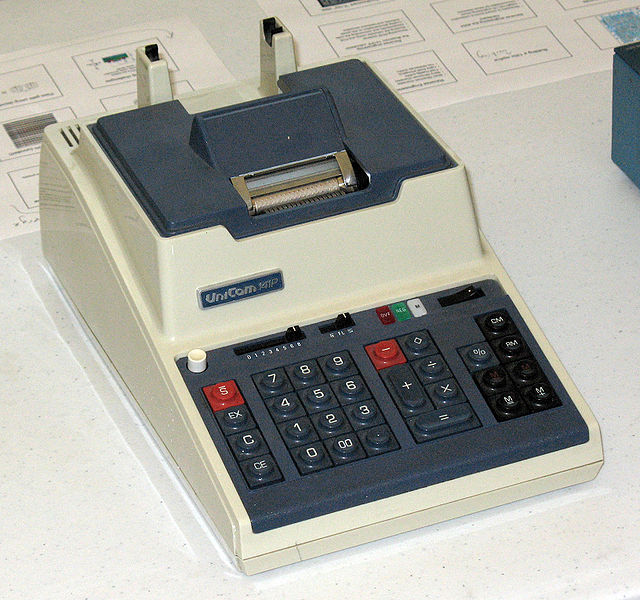
\includegraphics[width=.8\textwidth]{images/i4004-calculator.jpg}\\
    \begin{tiny}
      \emph{Unicom 141P Calculator 3} photo by Michael Holley.\\ 
    \end{tiny}
  \end{column}
\end{columns}
\end{frame}

\begin{frame}[t]{My first computer}
Sinclair ZX-Spectrum
\begin{columns}[T]
  \begin{column}{.7\textwidth}
    \begin{itemize}
      \item Zilog Z80 (1976).
        \begin{itemize}
          \item \textmark{Application domain}: Home computers, videoconsoles.
          \item \textmark{Technology}: 4,000 nm.
          \vfill
          \item \textenum{Data}:
            \begin{itemize}
              \item 8500 transistors.
              \item 2.5 MHz
              \item 5 Volts
            \end{itemize}
          \vfill
          \item \textenum{Features}:
            \begin{itemize}
              \item 8-bits data.
            \end{itemize}
      \end{itemize}
    \end{itemize}
  \end{column}
  \begin{column}{.3\textwidth}
    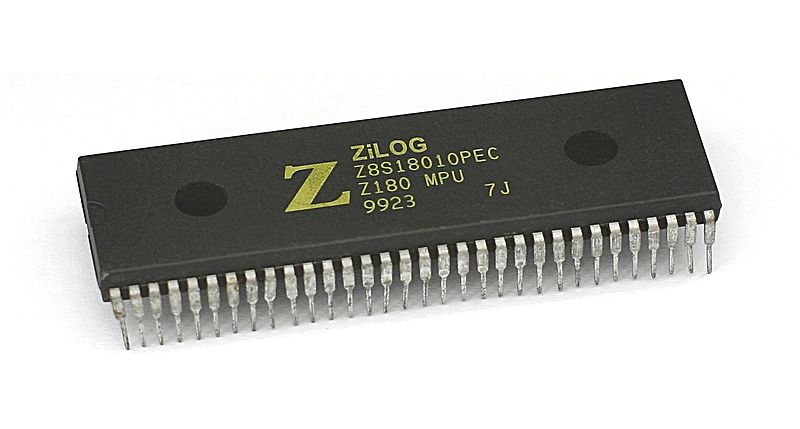
\includegraphics[width=.8\textwidth]{images/z80-micro.jpg}\\
    \begin{tiny}
      \emph{Zilog Z80} photo by Konstantin Lanzet\\
    \end{tiny}
    \vspace{1em}
    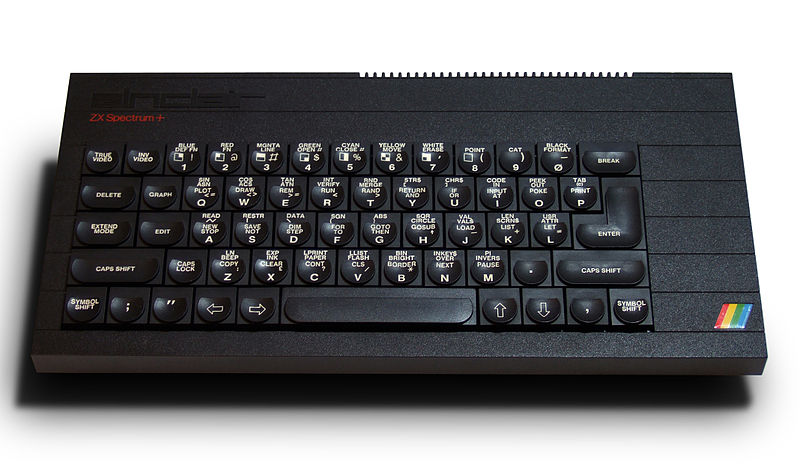
\includegraphics[width=.8\textwidth]{images/zx-spectrum.jpg}\\
    \begin{tiny}
      \emph{ZX Spectrum} photo by Bill Bertram.\\ 
    \end{tiny}
  \end{column}
\end{columns}
\end{frame}

%\begin{frame}[t]{My first PC}
%Intel 8088
%\end{frame}

\begin{frame}[t]{Last single core}
\vspace{-1em}
\begin{columns}
  \begin{column}{.15\textwidth}
    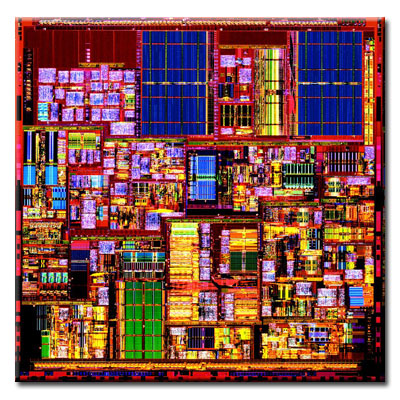
\includegraphics[width=\textwidth]{images/intel-p4-die.jpg}\\
    \begin{tiny}
      Die of Intel Pentium 4 (Northwood)\\ 
      Source: \url{http://gecko54000.free.fr}\\
    \end{tiny}
    \vspace{0.75em}
    \begin{center}
      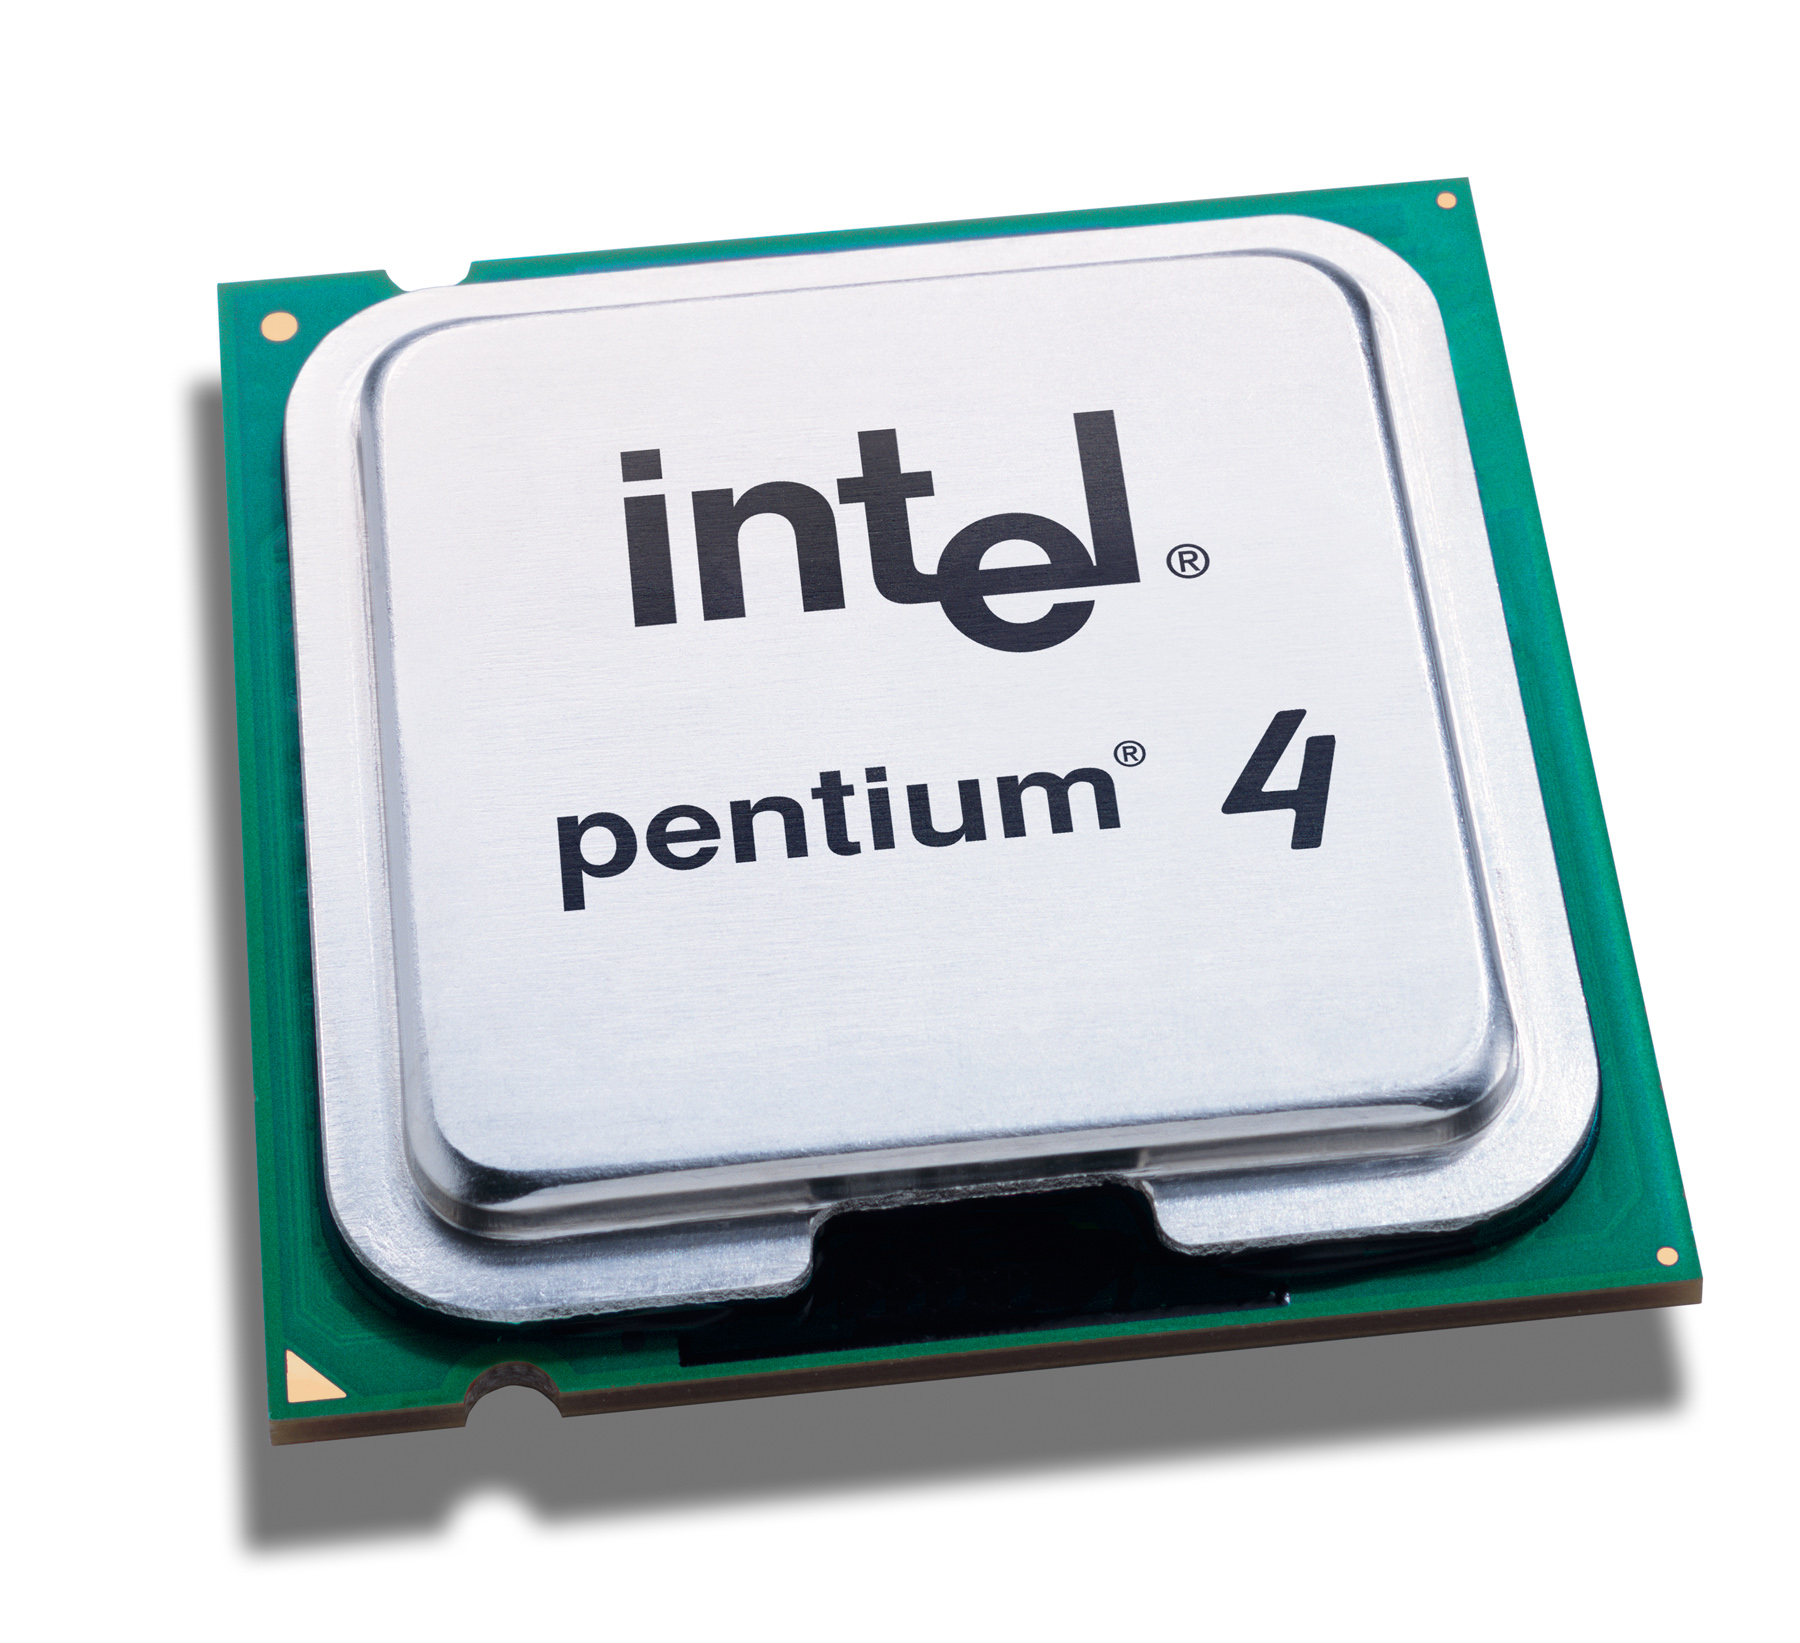
\includegraphics[width=.9\textwidth]{images/intel-p4.jpg}\\
    \end{center}
  \end{column}
  \begin{column}{.85\textwidth}
    \begin{itemize}
      \item Intel Pentium 4 (2003).
        \begin{itemize}
          \item \textmark{Application domain}: Desktop / Servers.
          \item \textmark{Technology}: 90 nm (1/100x).
        \end{itemize}
      \item \textenum{Data}:
        \begin{itemize}
          \item 55M transistors (20,000x).
          \item 101 mm$^2$ (10x).
          \item 3.4 GHz (10,000x).
          \item 1.2 Volts (1/10x).
        \end{itemize}
      \item \textenum{Features}:
        \begin{itemize}
          \item 32/64-bit data (16x).
          \item Data path with 22 pipeline stages (later 31).
          \item 3-4 instructions per cycle (superscalar).
          \item Two level cache on chip.
          \item Data parallel instructions (SIMD).
          \item Hyper-threading.
        \end{itemize}
    \end{itemize}
  \end{column}
\end{columns}
\end{frame}

\begin{frame}[t]{A typical multicore}
\vspace{-1em}
\begin{columns}
  \begin{column}{.7\textwidth}
    \begin{itemize}
      \item Intel Core i7 (2009).
        \begin{itemize}
          \item \textmark{Application}: Desktop / Server.
          \item \textmark{Technology}: 45 nm (1/2x).
        \end{itemize}
      \item \textenum{Data}:
        \begin{itemize}
          \item 774M transistors (12x).
          \item 296 mm$^2$ (3x).
          \item 3.2 GHz -- 3.6 GHz ($\approx$1x).
          \item 0.7 -- 1.4 Volts ($\approx$1x).
        \end{itemize}
      \item \textenum{Features}:
        \begin{itemize}
          \item 128-bit data (2x).
          \item Datapath with 14-stage pipeline (0.5x).
          \item 4 instructions per cycle ($\approx$1x).
          \item Three level cache on chip.
          \item Data parallel instructions (SIMD).
          \item 4 cores (4x) + Hyper-threading.
        \end{itemize} 
    \end{itemize}
  \end{column}
  \begin{column}{.35\textwidth}
    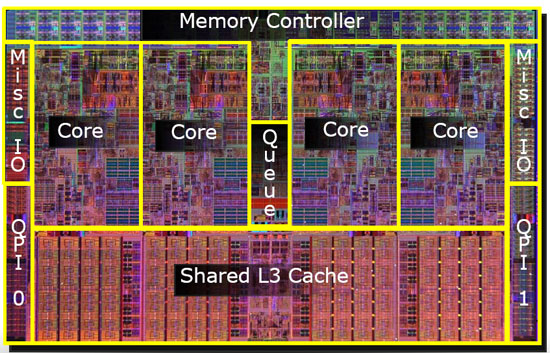
\includegraphics[width=\textwidth]{images/intel-core-i7-die.jpg}\\
    \begin{tiny}
      Die of Intel Core i7 (Nehalem)\\
      Source: \url{www.legitreviews.com}\\
    \end{tiny}
    \vspace{0.75em}
    \begin{center}
    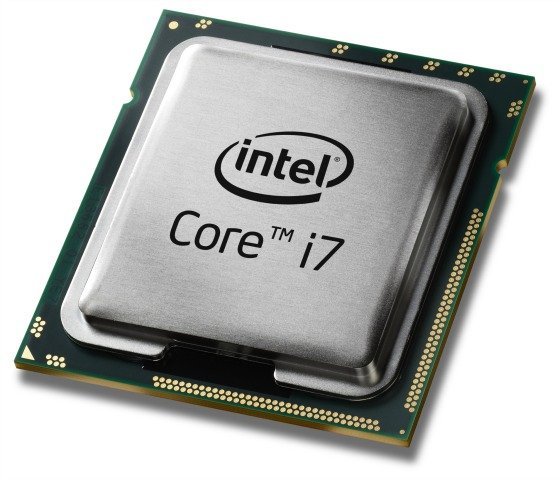
\includegraphics[width=.65\textwidth]{images/intel-core-i7.jpg}\\
    \end{center}
  \end{column}
\end{columns}
\end{frame}

\begin{frame}[t]{What happened?}
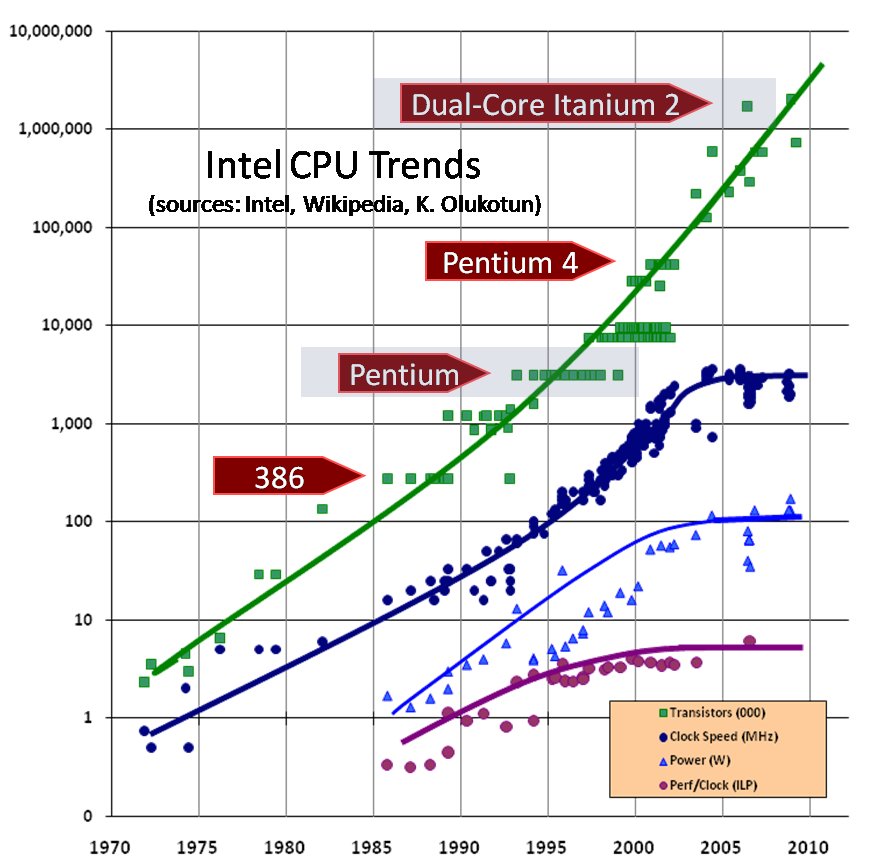
\includegraphics[height=.8\textheight,width=\textwidth]{images/free-lunch.png}\\
\begin{tiny}
Source: \alert{The free lunch is over}.
Herb Sutter.
\url{http://www.gotw.ca/publications/concurrency-ddj.htm}\\
\end{tiny}
\end{frame}

%\begin{frame}[t]{Hetorogeneity}
%\begin{itemize}
%  \item Welcome to the jungle!
%\end{itemize}
%\end{frame}
